\documentclass[12pt]{article}

\usepackage[utf8]{inputenc}
\usepackage[T1]{fontenc}
\usepackage{listings}
\usepackage{amsmath, amssymb}
\usepackage{graphicx}
\usepackage{hyperref}
\usepackage{geometry}
\usepackage{caption}
\usepackage{tcolorbox}
\usepackage{graphicx}
\usepackage{booktabs}
\usepackage{float}     % for the H placement specifier

\DeclareCaptionLabelFormat{customTable}{Tabela #2}
\captionsetup[table]{
    labelformat=customTable,
    labelsep=colon
}

\DeclareCaptionLabelFormat{customFigure}{Wykres #2}
\captionsetup[figure]{
    labelformat=customFigure,
    labelsep=colon
}

\geometry{a4paper, margin=1in}

\lstset{
    inputencoding=utf8x,
    extendedchars=\true,
    literate={ą}{{\k{a}}}1
             {Ą}{{\k{A}}}1
             {ę}{{\k{e}}}1
             {Ę}{{\k{E}}}1
             {ó}{{\'o}}1
             {Ó}{{\'O}}1
             {ś}{{\'s}}1
             {Ś}{{\'S}}1
             {ł}{{\l{}}}1
             {Ł}{{\L{}}}1
             {ż}{{\.z}}1
             {Ż}{{\.Z}}1
             {ź}{{\'z}}1
             {Ź}{{\'Z}}1
             {ć}{{\'c}}1
             {Ć}{{\'C}}1
             {ń}{{\'n}}1
             {Ń}{{\'N}}1
}


\title{Struktury Baz Danych Projekt 2 - Sprawozdanie z indeksowej organizacji plików z użyciem struktury B-drzewa}
\author{Kamil Szabłowski, 193248}
\date{\today}

\begin{document}

\maketitle

\section{Wprowadzenie}
Zadaniem projektu była implementacja jednego z wybranych algorytmów organizacji plików indeksowych.
Zaimplementowanym przeze mnie algorytmem jest algorytm \emph{B-drzewa}.

Użytym w projekcie typem rekordu pliku są ciągi 10 \emph{liczb} z dodatkowycm kluczem, 
będącym liczbą natruralną większą od 0. Kryterium sortowania rekordu jest wartość klucza.
Za \emph{liczbę} będącą elementem rekordu uznaję 32-bitową liczbę całkowita ze znakiem. 
Poniżej przedstawione został przykład takiego rekordu:

\[
\begin{array}{|c|c|c|c|c|c|c|c|c|c|c|}
\hline
1 & 23 & -45 & 67 & 12 & -8 & 34 & 0 & 29 & -16 & 5 \\
\hline
\end{array}
\]

Pierwszy element powyższego rekordu to kluczz wynoszący 1, reszta stanowi ciąg 10 liczb.

Rozmiar rekordu wynosi w takim razie 44 bajtów (11 liczb całkowitych 4-bajtowych).
Przyjęty rozmiar bloku dyskowego pliku danych na potrzeby tego eksperymentu wynosi 364 bajtów.


\section{Opis implementacji}
Użytą w tym projekcie metodą organizacji pliku jest użycie struktury B-drzewa.
\\\\
Alogorytmy wykorzystane do wstawianie, usuwania i wyszukiwania rekordów w B-drzewie są analogiczne do tych
przedstawionych na wykładzie.
Modyfikacja rekordu polega na usunięciu starego rekordu i dodaniu nowego rekordu z nowym kluczem, chyba że
nie dokonujemy zmiany klucza, wtedy modyfikowana jest wartość rekordu bezpośrednio w pliku z danymi, po uwczesnym
wyszukaniu klucza.
\\\\
W mojej implementacji na stronę B-drzewa zapisaną do pliku składają się:
\begin{itemize}
    \item Wskaźnik na stronę rodzica (liczba całkowita, 4B)
    \item Liczba rekordów w stronie (liczba całkowita, 4B)
    \item Lewy skrajny wskaźnik na stronę, z rekordami mniejszymi od wszystkich innych należących do obecnej strony (liczba całkowita, 4B)
    \item Od \(1\) do \(2d\) węzłów, gdzie na dany węzeł składa się:
    \begin{itemize}
        \item Wartość klucza rekordu (liczba całkowita, 4B)
        \item Offset rekordu o danym kluczu w pliku z danymi (liczba całkowita, 4B)
        \item Wskaźnik na stronę z rekordami większymi od klucza w tym węźle, ale mniejszymi od klucza w następnym węźle (liczba całkowita, 4B)
    \end{itemize}
\end{itemize}

Nie zależnie od ilości węzłów w pliku indeksowym B-drzewa, zapisana (lub odczytana) strona
z dysku ma zawsze rozmiar \(4+4+4+2d*12 = 12+24d\) bajtów.

Strona w pamięci w programie jest prawie identyczna jak strona zapisana na dysku, z tą różnicą, że
lewy skrajny wskaźnik na stronę jest zastąpiony dodatkowym węzłem 0, w którym poza wartością wskaźnika na 
stronę-dziecko, wartość klucza i rekordu ustawiona jest na NULL

Jeśli chodzi o plik z danymi, to podobnie jak w przypadku pierwszego projektu, 
rekordy są zapisywane binarnie, jeden po drugim, bez żadnych dodatkowych informacji.

\subsection{Opis buforowania}

Wykorzystane przeze mnie buforowanie polega na zapisywaniu do pamięci operacji, 
h+1 ostatnio używanych stron B-drzewa, gdzie h to wysokość drzewa.

Ważne jest jednak, że h stron bufora wykorzystywane jest w sposób normalny, opisany powyżej,
podczas gdy ostatnia strona bufora, ta o najniższym priorytecie (najstarsza),
ma specjalną funkcję.

Podczas zapisywania lub czytania strony, programistycznie możzna wskazać czy
operacja ta powinna być \texttt{lowPriority}. Jeśli tak, to strona ta jest zapisywana
na końcu bufora, a nie na początku, co oznacza, że zostanie ona usunięta jako pierwsza.
Jest to potrzebne by podczas operacji takich jak merge czy split, zachować w buforze
strony przez które się już przeszło. Mechanizm ten gwarantuje również, że root zawsze
znajduje się w pamięci, co znacząco zmniejsza liczbę operacji blokowych.
 
\section{Specyfikacja plików testowych}
Plikiem testowym jest plik tekstowy (.txt) o określonej poniżej strukturze.
\subsection{Struktura pliku testowego}
Plik testowy składa się z komend oddzielonych znakime nowej linii.
\\\\
Komendy dostępne do użycia w pliku testowym są analogiczne co do komend dostępnych w interfejsie tekstowym.
Lista dostępnych komend może zostać wyświetlona przy użyciu komendy \verb!help!. Dodatkowe komendy do debuggowania
programu są pokazane po użyciu komendy \verb!help debug!.
\\\\
Output komendy \verb!help!:

\begin{tcolorbox}[colframe=black!75, colback=white!95, title=Output komendy \texttt{help}]
\begin{verbatim}
List of available commands
TIP: Most commands can be used by using 
first letters of each word in the command
Example: 'am 5' is the same as 'addmulti 5'
--------------------------------------------------------------------
help                                     Show this help message
help debug                               Show help relating to debug
setcompensation [true/false]             Toggle compensation
clear                                    Clear all the files
rand [n]                                 Insert n random records
update [key] [value] [newKey: OPTIONAL]  Update record with given key
insert [key] [value]                     Insert record into the file
search [key]                             Search for record with key
print [group] [all]                      Prints all records in db
loadtest [filename]                      Loads test file
\end{verbatim}
\end{tcolorbox}

Output komendy \verb!help debug!:

\begin{tcolorbox}[colframe=black!75, colback=white!95, title=Output komendy \texttt{help debug}]
\begin{verbatim}
List of available debug commands
--------------------------------------------------------------------
dblockstats              Prints block stats
dforceflush              Forces a flush of the files
dgetrecord [n]           Gets a record at offset (data file)n
\end{verbatim}
\end{tcolorbox}


Przykład poprawnie ustrukturyzowanego pliku testowego:

\begin{tcolorbox}[colframe=black!75, colback=white!95, title=Plik: \texttt{text.txt}]
\begin{verbatim}
clear
insert 1 5
insert 2 10
insert 3 15
insert 4 20
insert 5 25
delete 2
search 3
search 2
dblockstats
print all group
print
\end{verbatim}
\end{tcolorbox}

Poniższy plik testowy wykona dokładnie to samo co powyższy:
\begin{tcolorbox}[colframe=black!75, colback=white!95, title=Plik: \texttt{text.txt}]
\begin{verbatim}
c
i 1 5
i 2 10
i 3 15
i 4 20
i 5 25
d 2
s 3
s 2
dbs
p a g
p
\end{verbatim}
\end{tcolorbox}

Tak spreparowany plik może bezproblemu zostać załadowany do interfejsu tekstowego.
\subsection{Załadowanie i uruchomienie pliku testowego}
Aby załadować plik testowy z dysku, wystarczy w interfejsie tekstowym użyć komendy \verb!loadtest nazwa_pliku.txt!,
gdzie zamiast \emph{nazwa\_pliku.txt} należy wpisać ścieżkę do docelowego pliku testowego, który ma zostać załadowany.
Ścieżka może być bezwzględna, lub względna - zależna od katalogu w którym został uruchomiony interfejs tekstowy.

\section{Sposób prezentacji wyników działania programu}

Po uruchomieniu programu, organizowany plik indeksowy orazz z danymi jest pusty i nie zawiera żadnych rekordów ani stron.

Aby dodać rekordy do bazy danych należzy użyć jednej z nastepujących komend:

\begin{itemize}
    \item \verb!insert [key] [value]! - próbuje dodać rekord o danym kluczu i wartości do bazy danych
    \item \verb!rand [n]! - próbuje dodać n losowych rekordów do bazy danych
\end{itemize}

Analogicznie, usunięcie rekordu z bazy danych odbywa się przy użyciu komendy \verb!delete [key]!.

Wyszukiwanie rekordu w bazie danych odbywa się przy użyciu komendy \verb!search [key]!.

Modyfikacja rekordu w bazie danych odbywa się przy użyciu komendy \verb!update [key] [value] [newKey: OPTIONAL]!

Po użyciu komendy \verb!print! bez żadnych parametrów, program wypisuje zawartość bazy danych w formie rekordów, od najmniejszego
do największego klucza w następującym formacie:
Przykład:
\begin{tcolorbox}[colframe=black!75, colback=white!95, title=Output komendy \texttt{print}]
\begin{verbatim}
(1) 10 10 10 10 10 10 10 10 10 10
(2) 20 20 20 20 20 20 20 20 20 20
(3) 30 30 30 30 30 30 30 30 30 30
(4) 40 40 40 40 40 40 40 40 40 40
(5) 50 50 50 50 50 50 50 50 50 50
\end{verbatim}
\end{tcolorbox}

Liczba w nawiasie to klucz rekordu, podczas gdy liczby po spacji to wartości rekordu, czyli liczby należące do ciągu.

Po użyciu komendy \verb!print! z parametrem \verb!group!, program wypisuje zawartość bazy danych w formie rekordów,
ale tym razem grupując rekordy znajdujące się na jednej stronie B-drzewa.

Po użyciu komendy \verb!print! z parametrem \verb!all!, program wypisuje zawartość bazy danych w pełnej formie. Przykład:
\begin{tcolorbox}[colframe=black!75, colback=white!95, title=Output komendy \texttt{print all}]
\begin{verbatim}
RecordOffset: 0 | PageOffset: 0 | ParentPageOffset: 1 
| LeftPagePtr: -1 | RightPagePtr: -1
(1) 1 1 1 1 1 1 1 1 1 1 

RecordOffset: 1 | PageOffset: 0 | ParentPageOffset: 1 
| LeftPagePtr: -1 | RightPagePtr: -1
(2) 2 2 2 2 2 2 2 2 2 2 

RecordOffset: 2 | PageOffset: 1 | ParentPageOffset: -1 
| LeftPagePtr: 0 | RightPagePtr: 2
(3) 3 3 3 3 3 3 3 3 3 3 

RecordOffset: 3 | PageOffset: 2 | ParentPageOffset: 1 
| LeftPagePtr: -1 | RightPagePtr: -1
(4) 4 4 4 4 4 4 4 4 4 4 

RecordOffset: 4 | PageOffset: 2 | ParentPageOffset: 1 
| LeftPagePtr: -1 | RightPagePtr: -1
(5) 5 5 5 5 5 5 5 5 5 5 

-----------------------------------
Total records: 5
Total pages count: 3
Height: 2
-----------------------------------
\end{verbatim}
\end{tcolorbox}

Poza wyświetleniem klucza i wartości rekordu, program wypisuje również informacje o stronach B-drzewa, 
takie jak:
\begin{itemize}
    \item \verb!RecordOffset! - offset rekordu w pliku z danymi
    \item \verb!PageOffset! - offset strony w pliku indeksowym
    \item \verb!ParentPageOffset! - offset strony rodzica w pliku indeksowym
    \item \verb!LeftPagePtr! - offset strony dziecka z rekordami mniejszymi od klucza w obecnym węźle
    \item \verb!RightPagePtr! - offset strony dziecka z rekordami większymi od klucza w obecnym węźle
\end{itemize}

Wartość \(-1\) w polach \verb!LeftPagePtr!, \verb!RightPagePtr! oraz \verb!ParentPageOffset! oznacza, 
że dany wskaźnik nie wskazuje na nic, czyli węzeł nie ma dzieci, bądź rodzica (tylko korzeń).

Dodatkowo wyświetlana jest informacja o całkowitej liczbie rekordów, 
liczbie stron oraz wysokości drzewa.


Po użyciu komendy \verb!print all group! program wypisuje zawartość bazy danych w pełnej formie, 
ale tym razem grupując rekordy po stronach B-drzewa. Przykład:
\begin{tcolorbox}[colframe=black!75, colback=white!95, title=Output komendy \texttt{print all group}]
\begin{verbatim}
-------- Page 0 ----------
RecordOffset: 0 | PageOffset: 0 | ParentPageOffset: 1 
| LeftPagePtr: -1 | RightPagePtr: -1
(1) 1 1 1 1 1 1 1 1 1 1 

RecordOffset: 1 | PageOffset: 0 | ParentPageOffset: 1 
| LeftPagePtr: -1 | RightPagePtr: -1
(2) 2 2 2 2 2 2 2 2 2 2 

-------- Page 1 ----------
RecordOffset: 2 | PageOffset: 1 | ParentPageOffset: -1 
| LeftPagePtr: 0 | RightPagePtr: 2
(3) 3 3 3 3 3 3 3 3 3 3 

-------- Page 2 ----------
RecordOffset: 3 | PageOffset: 2 | ParentPageOffset: 1 
| LeftPagePtr: -1 | RightPagePtr: -1
(4) 4 4 4 4 4 4 4 4 4 4 

RecordOffset: 4 | PageOffset: 2 | ParentPageOffset: 1 
| LeftPagePtr: -1 | RightPagePtr: -1
(5) 5 5 5 5 5 5 5 5 5 5 

-----------------------------------
Total records: 5
Total pages count: 3
Height: 2
-----------------------------------
\end{verbatim}
\end{tcolorbox}

Jak widać powyżej, rekordy są grupowane po stronach B-drzewa, co w przypadku większej ilości rekordów może spowodować,
że rekordy nie są wyświetlone w kolejności rosnącej klucza.

\section{Eksperyment}
\subsection{Konstrukcja eksperymentu}
Do przeprowadzenia eksperymentu wykorzystane zostały funkcje udostępniane prze interfejs
tekstowy programu.

Schemat eksperymentu wyglądał następująco:

\begin{enumerate}
    \item Ustawienie parametru D B-drzewa zgodnie z przeprowadzanym eksperymentem i kompilacja programu
    \item Wprowadzenie komend ręcznie do interfejsu tekstowego
    \item Spisanie informacji o każdej operacji do pliku tekstowego
    \item Wygenerowanie wykresów na podstawie danych eksperymentalnych
    \item Analiza otrzymanych wyników
\end{enumerate}

\subsection{Przygotowania do eksperymentu}

Zmiana parametru D B-drzewa odbywa się poprzez zmianę wartości stałej zdefiniowanej w pliku \texttt{defines.h}
jako \verb!BTREE_D_FACTOR!.
\\\\
Eksperyment polegający na wstawieniu N losowych rekordów do pliku, i spisaniu ich wyników został przeprowadzony
przez wpisanie kolejnych komend:
\begin{verbatim}
    clear
    rand N
    dblockstats
    print all group
\end{verbatim}
Gdzie N to liczba rekordów, którą chcemy wstawić do pliku.

Na potrzeby tego eksperymentu, N przyjmowało wartości od \(N = \{250, 1000, 2500, 10000, 25000 \} \),
a współczynnik D B-drzewa przyjmował wartości \(D = \{2, 4, 6, 10, 20, 50 \}\).
\\\\
Wyniki eksperymentu zostały zapisane do pliku tekstowego \texttt{eksperyment.txt}.
Wyniki te następnie zostały użyte do utwożenia wykresów i tabel, które zostały przedstawione w kolejnej sekcji.

\subsection{Wyniki eksperymentu}

\subsubsection{Liczba operacji blokowych}
\begin{table}[H]
\centering
\caption{Średnia liczba operacji blokowych dla różnych wartości D, przy wstawianiu 10000 rekordów}
\begin{tabular}{|c|c|c|c|c|c|}
\hline
D & Odczyty & Zapisy & Średnia liczba operacji na rekord & Wysokość \\
\hline
2 & 68451 & 30452 & 9.8982 & 7 \\
4 & 49086 & 24137 & 7.3252 & 5 \\
6 & 39877 & 21114 & 6.1009 & 4 \\
10 & 30853 & 18198 & 4.9080 & 4 \\
20 & 21809 & 15135 & 3.6959 & 3 \\
50 & 12230 & 11838 & 2.4075 & 3 \\
\hline
\end{tabular}
\end{table}

\begin{figure}[H]
    \centering
    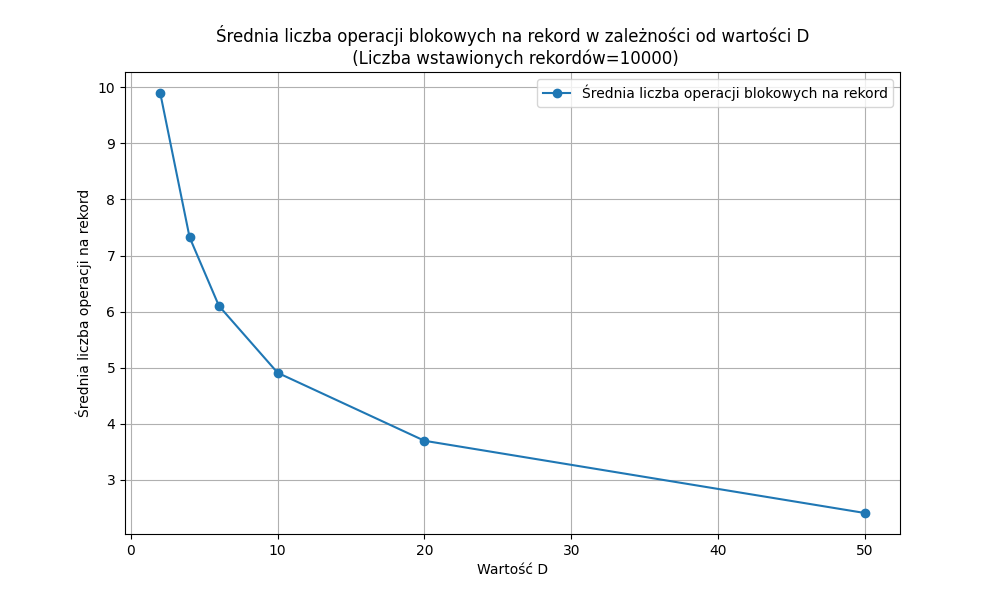
\includegraphics[width=\textwidth]{../Plots/block_operations_per_record.png}
    \caption{Średnia liczba operacji blokowych przypadających na pojedynczy rekord}
    \label{fig:plot1}
\end{figure}

Jak widać z powyższego wykresu, zwiększenie wartości D B-drzewa powoduje 
zmniejszenie liczby odczytów i zapisów blokowych przypadających na pojedynczy rekord, 
co świadczy o lepszej efektywności działania B-drzewa.

Z tabelki można również przeczytać, że zwiększenie wartości D B-drzewa 
powoduje zmniejszenie wysokości drzewa.
Biorąc to pod uwagę można stwierdzić, że średnia liczba operacji blokowych na B-drzewie
jest odwrotnie proporcjonalna do wysokości tego drzewa.

\subsubsection{Wypełnienie B-drzewa na dysku}

\begin{table}[H]
\centering
\caption{Wypełnienie pliku indeksowego B-drzewa na dysku dla różnych wartości D, przy wstawianiu 10000 rekordów}
\begin{tabular}{|c|c|c|c|}
\hline
D & Rozmiar rekordu (B) & Całkowity rozmiar drzewa(B) & Wypełnienie drzewa (\%) \\
\hline
2 & 119904 & 184800 & 64.88 \\
4 & 119952 & 163512 & 73.36 \\
6 & 119964 & 156468 & 76.67 \\
10 & 119928 & 151200 & 79.32 \\
20 & 119952 & 144648 & 82.93 \\
50 & 119964 & 144228 & 83.18 \\
\hline
\end{tabular}
\end{table}

\begin{figure}[H]
    \centering
    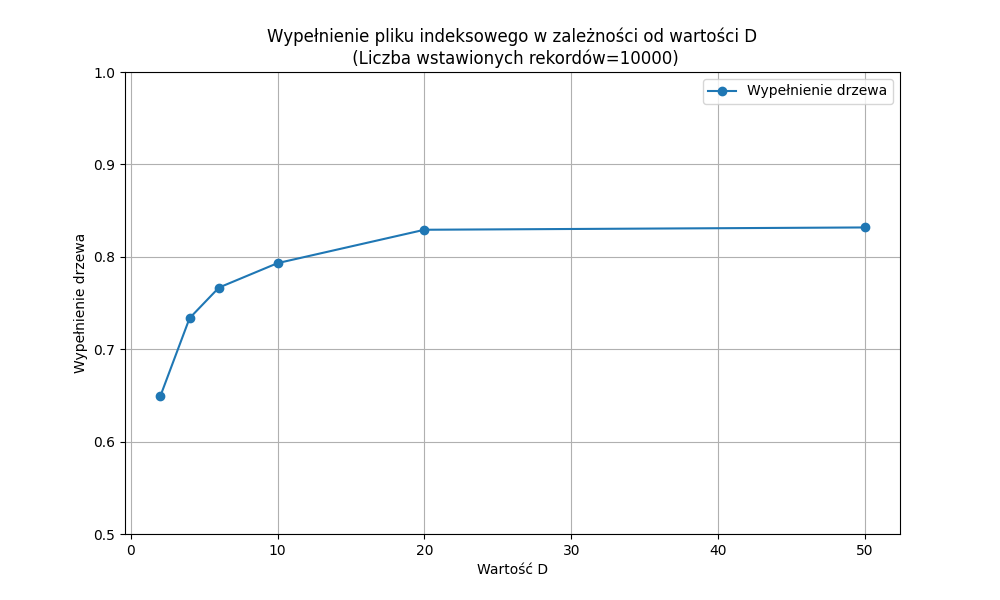
\includegraphics[width=\textwidth]{../Plots/tree_fill.png}
    \caption{Wypełnienie pliku indeksowego na dysku}
    \label{fig:plot2}
\end{figure}

Wyniki można odczytać tak, że na jeden rekord faktycznie zapisany w strukturze logicznej
B-drzea przypada X\% rekordu zapisanego na dysku.

Z powyższego wykresu można zauważyć, że zwiększenie wartości parametru D B-drzewa powoduje
również zwiększenie poziomu wypełnienia pliku indeksowego na dysku. Wzrost ten jest
znaczący dla małych wartości D, ale dla większych wartości D, dochodzi do stagnacji wypełnienia
pliku na dysku.
\\\\
Wynika z tego, że optymalne wartości parametru D dla B-drzewa
nie powinny być bardzo małe, gdyż wtedy plik indeksowy na dysku jest wypełniony bardziej nieefektywnie,
niż dla dużych waartości.

\subsubsection{Ilość dodawanych rekordów}
\begin{table}[H]
\centering
\caption{Liczba operacji blokowych dla różnych ilości rekordów}
\begin{tabular}{|c|c|c|}
\hline
Liczba rekordów & D = 2 & D = 10 \\
\hline
250 & 1598 & 472 \\
1000 & 8045 & 3067 \\
2500 & 21675 & 10126 \\
10000 & 98545 & 48649 \\
25000 & 261268 & 133576 \\
\hline
\end{tabular}
\end{table}

\begin{figure}[H]
    \centering
    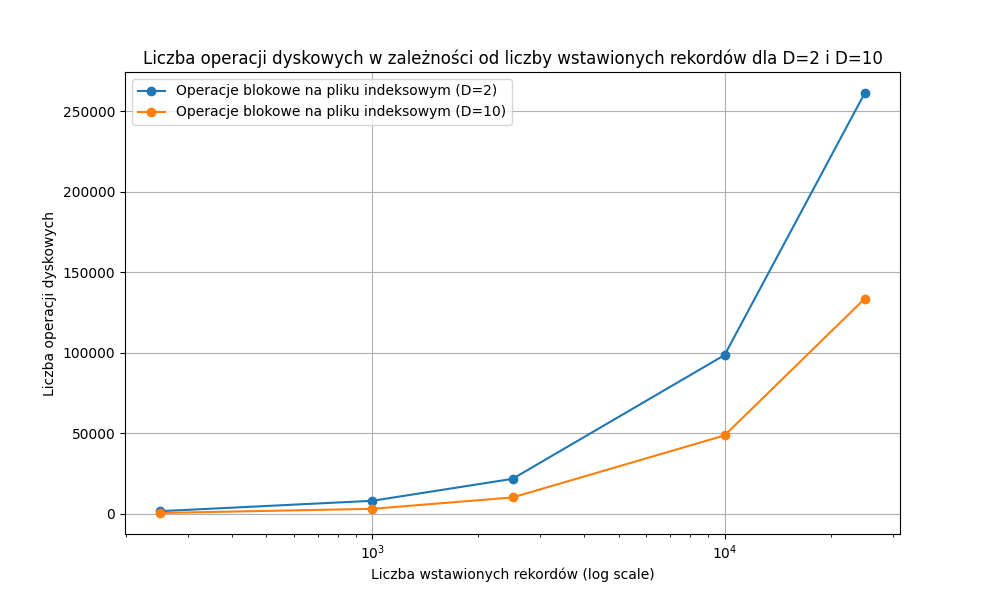
\includegraphics[width=\textwidth]{../Plots/disk_operations_by_record_count.png}
    \caption{Liczba operacji blokowych w zależności od ilości rekordów}
    \label{fig:plot3}
\end{figure}

Jak widać na powyższym wykresie, zzarówno liczba dodawanych rekordów jak i parametr D ma wpływ 
na liczbę wykonywanych operacji blokowych na B-drzewie. 

Zwiększenie liczby rekordów powoduje szybszy od liniowego wzrost liczby operacji blokowych,
co można wyjaśnić faktem, że dla większej ilości rekordów w B-drzewie,
istnieje możliwość że wysokość drzewa wzrosła, a operacje na większym drzewie
wymagają przynajmniej o jedną więcej operację blokową na operacje na rekordzie.

Można też zauważyć, że dla większego D=10, liczba operacji blokowych jest mniejsza od D=2,
ale mimo to kształt obu wykresów jest bardzo podobny.


\end{document}